% !TeX spellcheck = de_DE

\chapter{Evaluation of the Tool}\label{evaluation} 
This chapter gives detailed information on how our tool is evaluated. Evaluation of the tool is done on the basis of parameters used by similar tools to access the quality of generated test scripts. These parameters facilitate correlating our tool with other tools.

The first section of the chapter speaks on the various methods and criteria used for evaluation. The second section of this chapter discusses the different results obtained from the evaluation and also compares our tool with similar tools available in the research domain.
\section{Preliminary Preparation for Evaluation}
This section gives an idea of the system to be used for evaluation, the different criteria and the procedure used for evaluation.
\subsection{System for Evaluation}
For evaluation of \gls{tsgt} tool, we use a system called \gls{lms}. The \gls{lms} is safety critical automotive software used in most of the present-day automobiles. The \glspl{srs} for \gls{lms} provided in \cite{blazysoftware} serves a foundation for our evaluation. This document provides an overview of the entire system and the various requirements needed for system development.  It also provides detailed requirements for specific functionalities and in addition, includes models describing the functionality and interactions of the system. The requirements are organized in the form of use cases and there are totally 13 use cases which act as inputs for our tool.
\subsection{Evaluation Criteria}\label{criteria}
The evaluation of the tool is based on two main criteria.
\begin{enumerate}
\item The time taken for the generation of test scripts.
\item The coverage of requirements by the generated test cases.
\end{enumerate}
\subsubsection{\textbf{Time Criteria}} 

\begin{definition}
\label{def:def5}

The effort required to generate a test case is defined as the average time taken to generate the test cases \cite{elghondakly2015waterfall}.

Effort$_{TC}$   = $\displaystyle\frac{\mbox{Time taken to generate the test cases}}{\mbox{Total number of generated test cases}}$

In case of the automated process, the time taken to generate the test cases is inclusive of the time that is required to specify the requirements in \gls{rnl}, whereas in case of the manual process, it is inclusive of the time taken to convert the test cases into executable test scripts.
\end{definition}

\begin{definition}
\label{def:def6}

Test Case Productivity is defined as the ratio of the number of test steps generated to the time taken (in minutes) to generate these test steps \cite{gulechha2009software}.

Test Case Productivity (TCP)   = $\displaystyle\frac{\mbox{Number of test steps generated}}{\mbox{Total Time taken to generate the test steps}}$
\end{definition}

\subsubsection{\textbf{Coverage Criteria}}
The following criterion is necessary to analyze the quality of the test case generation process. This criterion also evaluates our methodology for Petri Net derivation since the test case generation depends upon the derived Petri Net.

\begin{definition}
\label{def:def7}

The generated test cases must ensure that all the requirements in \gls{srs} are covered at least once. This is also a requirement of ISO-26262 \cite{iso201126262}, a standard for functional safety of automobiles.

Requirement Coverage = $\displaystyle\frac{\mbox{Number of requirements covered}}{\mbox{Number of requirements present in the \gls{srs}}}$  $\times 100$
\end{definition}

\begin{definition}
\label{def:def8}

The generated test cases must ensure that all possible paths from the initial place to the final place in a Petri Net are covered at least once.

Path Coverage = $\displaystyle\frac{\mbox{Number of paths covered}}{\mbox{Number of paths present}}$  $\times 100$
\end{definition}

\subsection{Evaluation Procedure}
The sequence of steps followed for evaluation of the tool is shown graphically in Figure \ref{fig:chap6fig1}. The evaluation is done by comparing the manual and automatic generation of test scripts. The \gls{srs} document provided in \cite{blazysoftware} acts as input for the domain expert. In case of manual means, the domain expert analysis the \gls{srs} document and creates the test specification. Once it is done, the tester creates the test scripts corresponding to the test specification. In case of automatic means, the domain expert writes the requirements in \gls{rnl} and provides it as an input to the \gls{tsgt} tool which directly generates the test scripts.

\begin{figure}[htb!]
\centering
\fbox{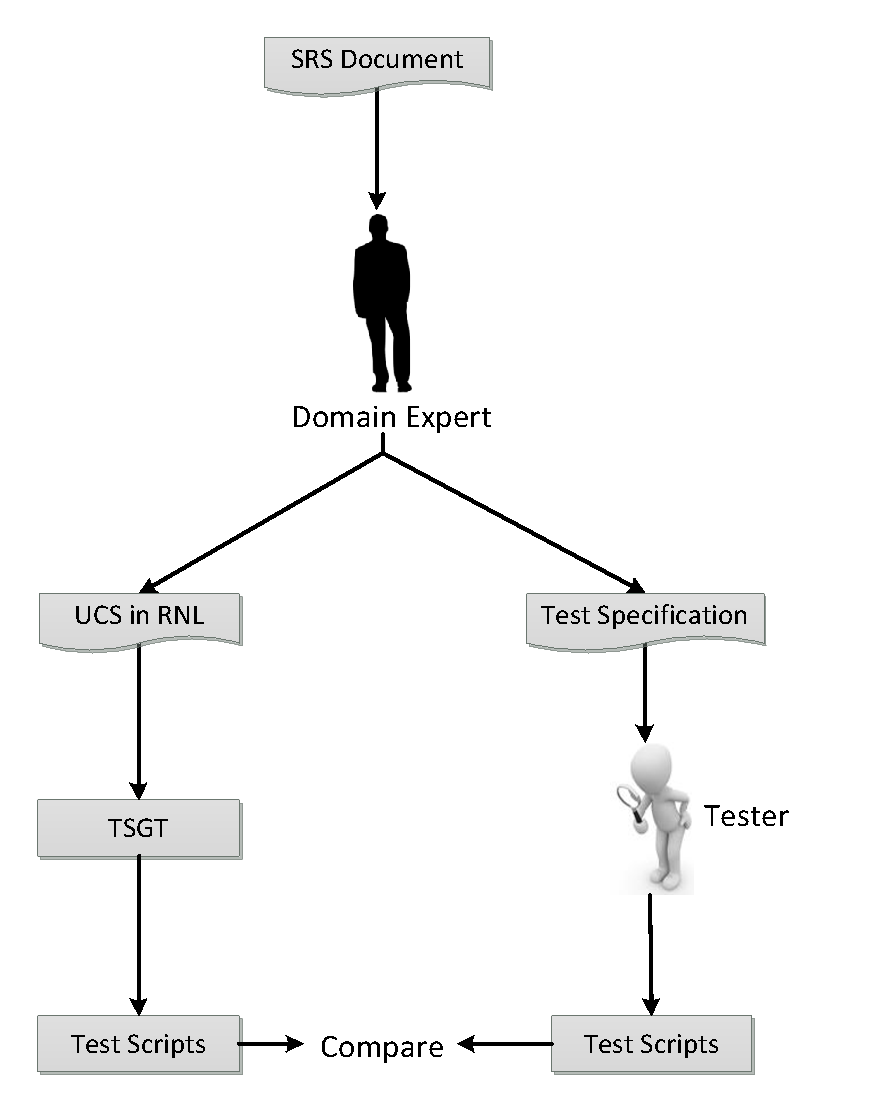
\includegraphics[scale=0.7]{content/images/Chapter6/figure1.pdf}}
\caption{The procedure used for evaluating the tool}
\label{fig:chap6fig1}
\end{figure}

\section{Evaluation Results and Discussion}
This section lists out the results obtained from the evaluation process and further discusses the various inferences from the results.
\subsection{Analysis of Quantitative Data}
\subsubsection{Based on Time Criteria}
The results of the tool evaluation are first discussed with respect to time criteria discussed in Section \ref{criteria} . Table \ref{tab:manualresults} and \ref{tab:toolresults} describe the different parameters for manual and tool generated test scripts respectively. The tables provide data of five different use cases from our evaluation system and also the average of different parameters.

% Table generated by Excel2LaTeX from sheet 'Sheet4'
\begin{table}[htbp]
  \centering
  \caption{Evaluation results from manual test script generation}
  	\begin{adjustbox}{width=1\textwidth}
    \begin{tabular}{|l|c|c|c|c|c|c|}
    \toprule
    \multicolumn{1}{|c|}{\multirow{2}[4]{*}{\textbf{Manual}}} & \multicolumn{6}{c|}{\textbf{Use Case }} \\
\cmidrule{2-7}          & \textbf{1} & \textbf{2} & \textbf{3} & \textbf{4} & \textbf{5} & \textbf{Average} \\
    \midrule
    \textit{\textbf{Total Time Taken (Manual)}} & 40    & 45    & 60    & 50    & 75    & 54.0 \\
    \midrule
    \textit{\textbf{Number of test cases (Manual) }} & 3     & 5     & 6     & 5     & 7     & 5 \\
    \midrule
    \textit{\textbf{Effort$ _{\textbf{TC}}$}} & 13.3  & 9.0   & 10.0  & 10.0  & 10.7  & 10.6 \\
    \midrule
    \textit{\textbf{Number of test steps}} & 24    & 32    & 34    & 34    & 45    & 34 \\
    \midrule
    \textit{\textbf{Test Case Productivity (TCP)}} & 0.6   & 0.7   & 0.6   & 0.7   & 0.6   & 0.6 \\
    \bottomrule
    \end{tabular}%
    \end{adjustbox}
  \label{tab:manualresults}%
\end{table}%


% Table generated by Excel2LaTeX from sheet 'Sheet4'
\begin{table}[htbp]
  \centering
  \caption{Evaluation results from automatic test script generation}
  	\begin{adjustbox}{width=1\textwidth}
    \begin{tabular}{|l|c|c|c|c|c|c|}
    \toprule
    \multicolumn{1}{|c|}{\multirow{2}[4]{*}{\textbf{TSGT}}} & \multicolumn{6}{c|}{\textbf{Use Case }} \\
\cmidrule{2-7}          & \textbf{1} & \textbf{2} & \textbf{3} & \textbf{4} & \textbf{5} & \textbf{Average} \\
    \midrule
    \textit{\textbf{Total Time Taken (TSGT)}} & 10    & 10    & 15    & 12    & 18    & 13.0 \\
    \midrule
    \textit{\textbf{Number of test cases (TSGT)}} & 5     & 7     & 9     & 8     & 12    & 8 \\
    \midrule
    \textit{\textbf{Effort$ _{\textbf{TC}}$}} & 2.0   & 1.4   & 1.7   & 1.5   & 1.5   & 1.6 \\
    \midrule
    \textit{\textbf{Number of test steps}} & 30    & 45    & 52    & 52    & 78    & 51 \\
    \midrule
    \textit{\textbf{Test Case Productivity (TCP)}} & 3.0   & 4.5   & 3.5   & 4.3   & 4.3   & 3.9 \\
    \bottomrule
    \end{tabular}%
    \end{adjustbox}
  \label{tab:toolresults}%
\end{table}%


According to Definition \ref{def:def5}, effort per test case is indicative of the average time required to generate each test case. The tables show that the effort required for each test case in the manual method is 10.6 minutes per test case on an average whereas in the automatic generation it is 1.6 minutes per test case. This denotes an 85\% improvement over the manual method.

\begin{figure}[htb!]
\centering
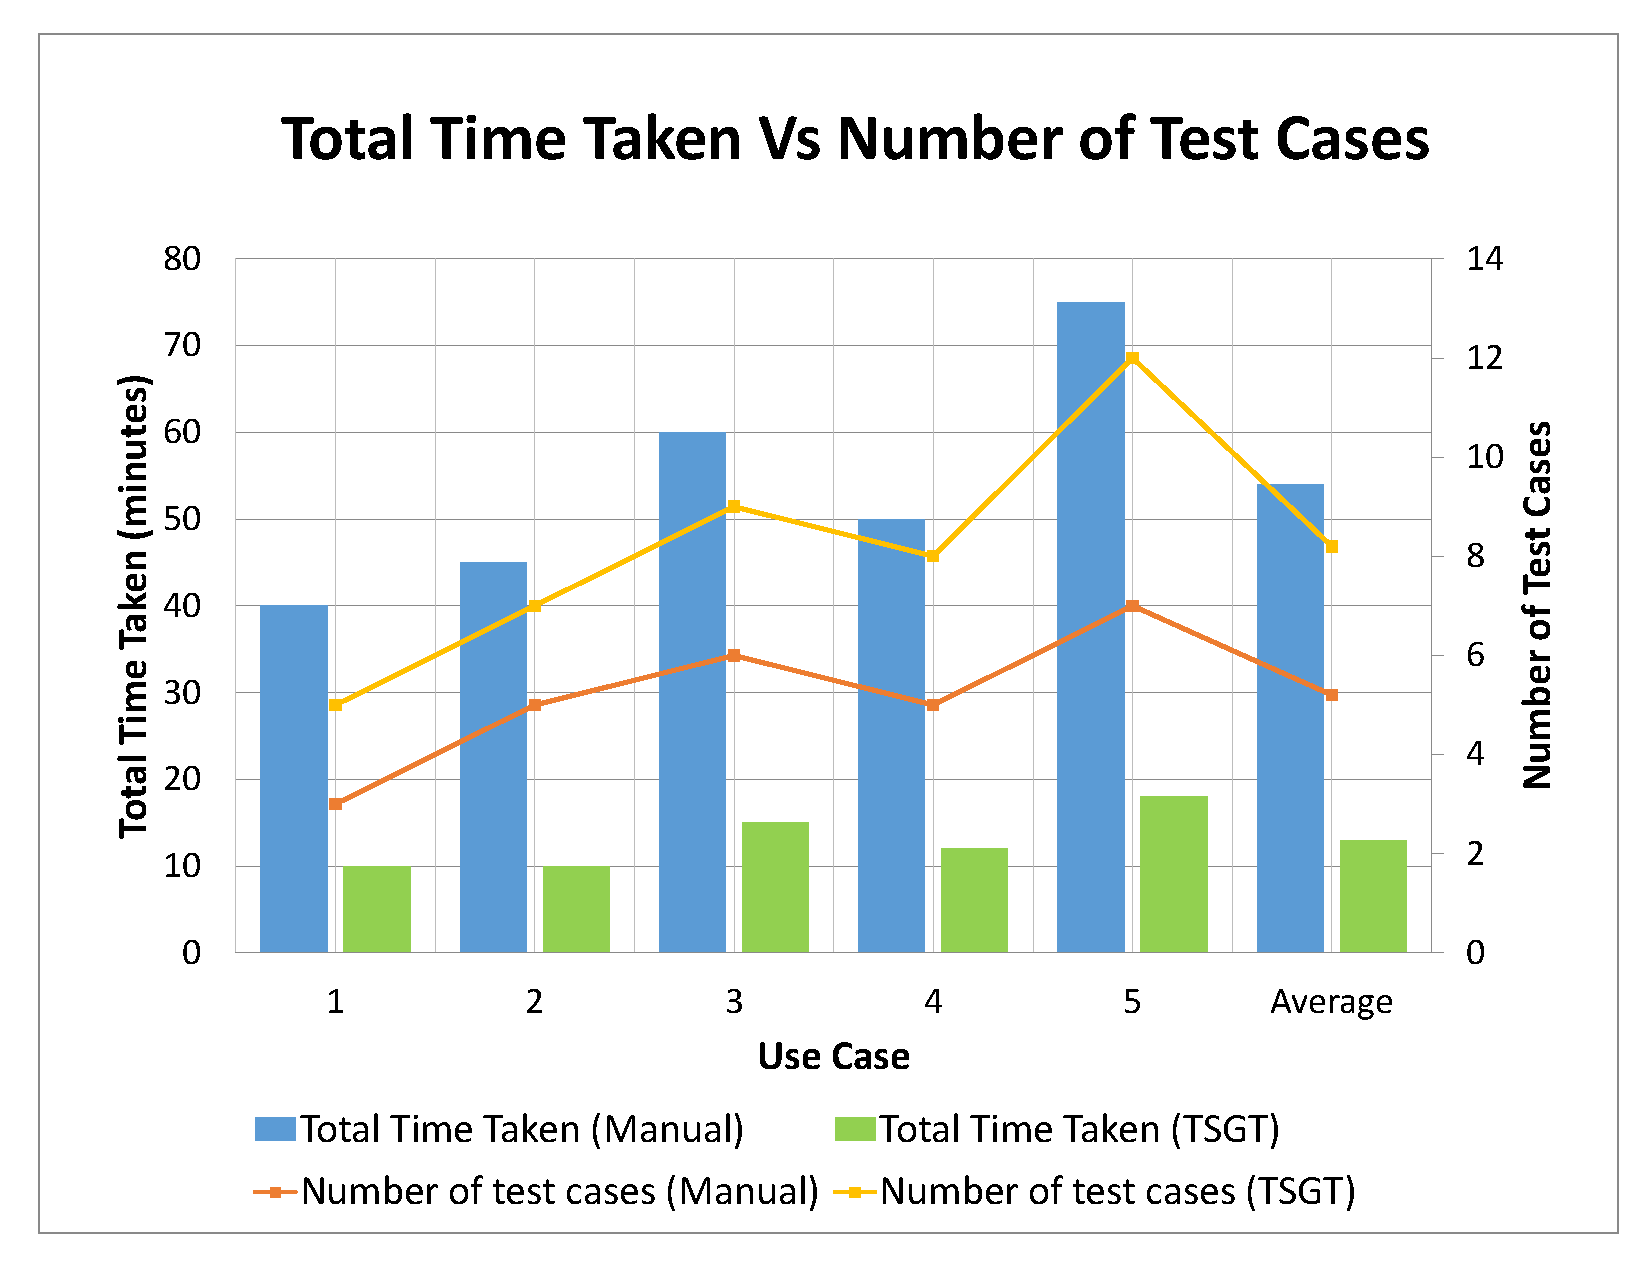
\includegraphics[scale=0.45]{content/images/Chapter6/figure2.pdf}
\caption{Effort\textsubscript{TC} and TCP for manual and automatic method}
\label{fig:chap6fig2}
\end{figure}

According to Definition \ref{def:def6}, \gls{tcp} shows the number of test steps that can be generated in one minute. From the tables, it can be seen that our tool generated 3.3 more test steps in a minute because \gls{tcp} stands at 0.6 and 3.9 for manual and automatic methods respectively. Figure \ref{fig:chap6fig2} shows a chart that contains the details of all the individual use cases.
From the tables, it can be inferred that the total time taken for generating the test scripts manually takes 54 minutes on an average whereas the total time taken for automatic test script generation is only 13 minutes. This implies that there is a 76\% reduction in time when the tool is used for test script generation.

\subsubsection{Based on Coverage Criteria}

This segment deals with the results of the tool evaluation based on coverage criteria discussed in Section \ref{criteria}. Table \ref{tab:coverageresults} describes the different parameters for manual and tool generated test scripts respectively.
% Table generated by Excel2LaTeX from sheet 'Sheet7'
\begin{table}[htbp]
  \centering
  \caption{Evaluation results of coverage criteria}
  	\begin{adjustbox}{width=1\textwidth}
    \begin{tabular}{|l|c|c|c|c|c|c|}
    \toprule
    \multicolumn{1}{|c|}{\multirow{2}[4]{*}{\textbf{Parameters}}} & \multicolumn{6}{c|}{\textbf{Use Case }} \\
\cmidrule{2-7}          & \textbf{1} & \textbf{2} & \textbf{3} & \textbf{4} & \textbf{5} & \textbf{Average} \\
    \midrule
    \textit{\textbf{Number of test cases (Manual)}} & 3     & 5     & 6     & 5     & 7     & 5.2 \\
    \midrule
    \textit{\textbf{Requirement Coverage  (Manual)}} & 60\%  & 80\%  & 85\%  & 90\%  & 70\%  & 77\% \\
    \midrule
    \textit{\textbf{Path Coverage  (Manual)}} & 100\% & 90\%  & 85\%  & 70\%  & 90\%  & 87\% \\
    \midrule
    \textit{\textbf{Number of test cases  (TSGT)}} & 5     & 7     & 9     & 8     & 12    & 8.2 \\
    \midrule
    \textit{\textbf{Requirement Coverage (TSGT)}} & 100\% & 100\% & 100\% & 100\% & 100\% & 100\% \\
    \midrule
    \textit{\textbf{Path Coverage (TSGT)}} & 100\% & 100\% & 100\% & 100\% & 100\% & 100\% \\
    \bottomrule
    \end{tabular}%
    \end{adjustbox}
  \label{tab:coverageresults}%
\end{table}%

From the table, it can be inferred that the number of test cases generated by manual method is always less than the automatic method. The coverage percentage in case of manual method is solely dependent on the individual extracting the test cases. Hence we see a difference in coverage percentage in manual method and it is arbitrary. But in the automatic method, requirement and path coverage are always 100\%. This is due to the formal method of test case generation and this also ensures that each requirement and path is covered with the generated test cases. 

\subsection{Discussion of the Results}
This section compares our tool i.e. \gls{tsgt} with other closely related test script generation tools available in the research field. Figure \ref{fig:chap6fig3} shows a graphical representation of the comparison between different approaches based on the effort per test case criterion. The data for the manual and \gls{tsgt} approach is taken out from our evaluation. \cite{yue2015rtcm}provides the data for \gls{rtcm} and \gls{umtg} approach.

The pros and cons of the different approaches are discussed below. \gls{umtg} provides an exhaustive test data for test script generation but it requires domain models for test data generation. The need for domain model generation along with test data generation using \gls{ocl} increases the effort required for test case generation. \gls{rtcm} provides the best solution but it requires manual intervention to improve some of the intermediate artifacts which might increase the effort in some cases. 

\begin{figure}[htb!]
\centering
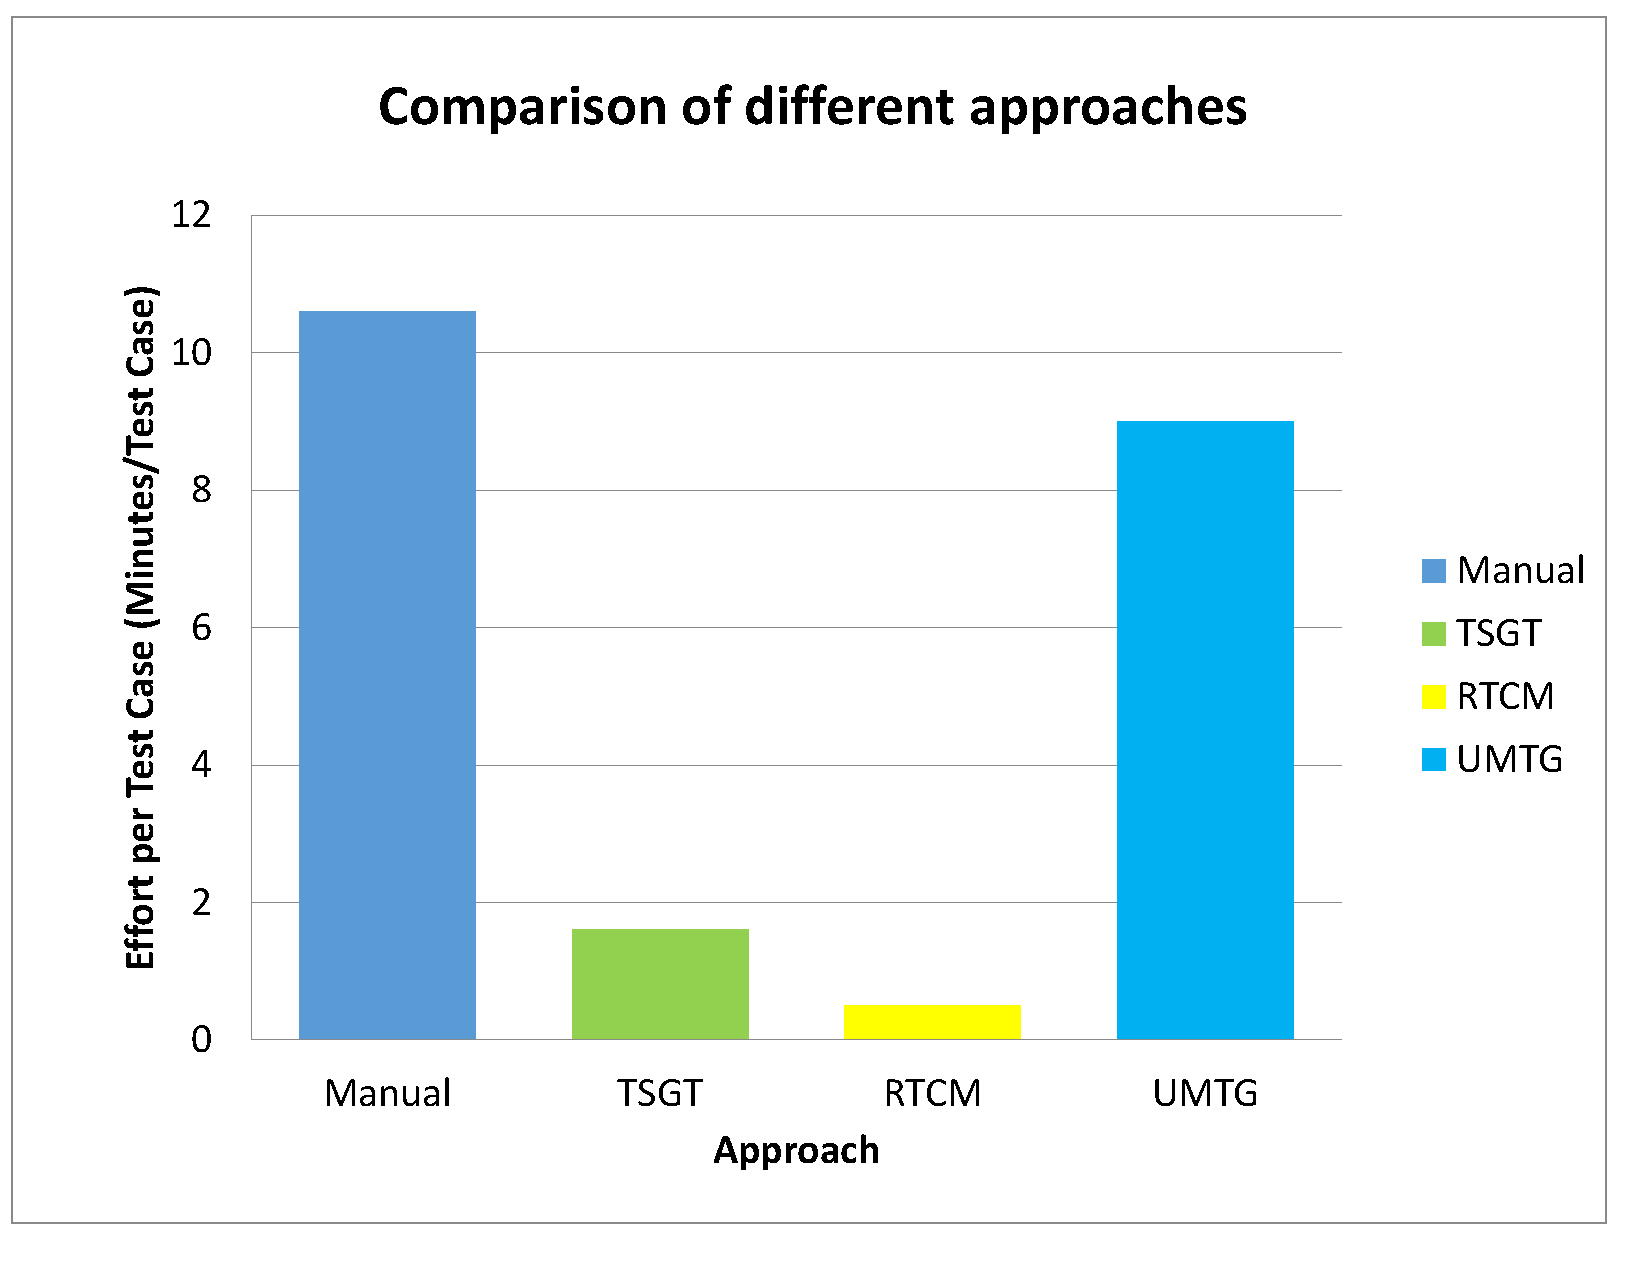
\includegraphics[scale=0.45]{content/images/Chapter6/figure3.pdf}
\caption{Comparison between different existing approaches}
\label{fig:chap6fig3}
\end{figure}


\begin{figure}[htb!]
\centering
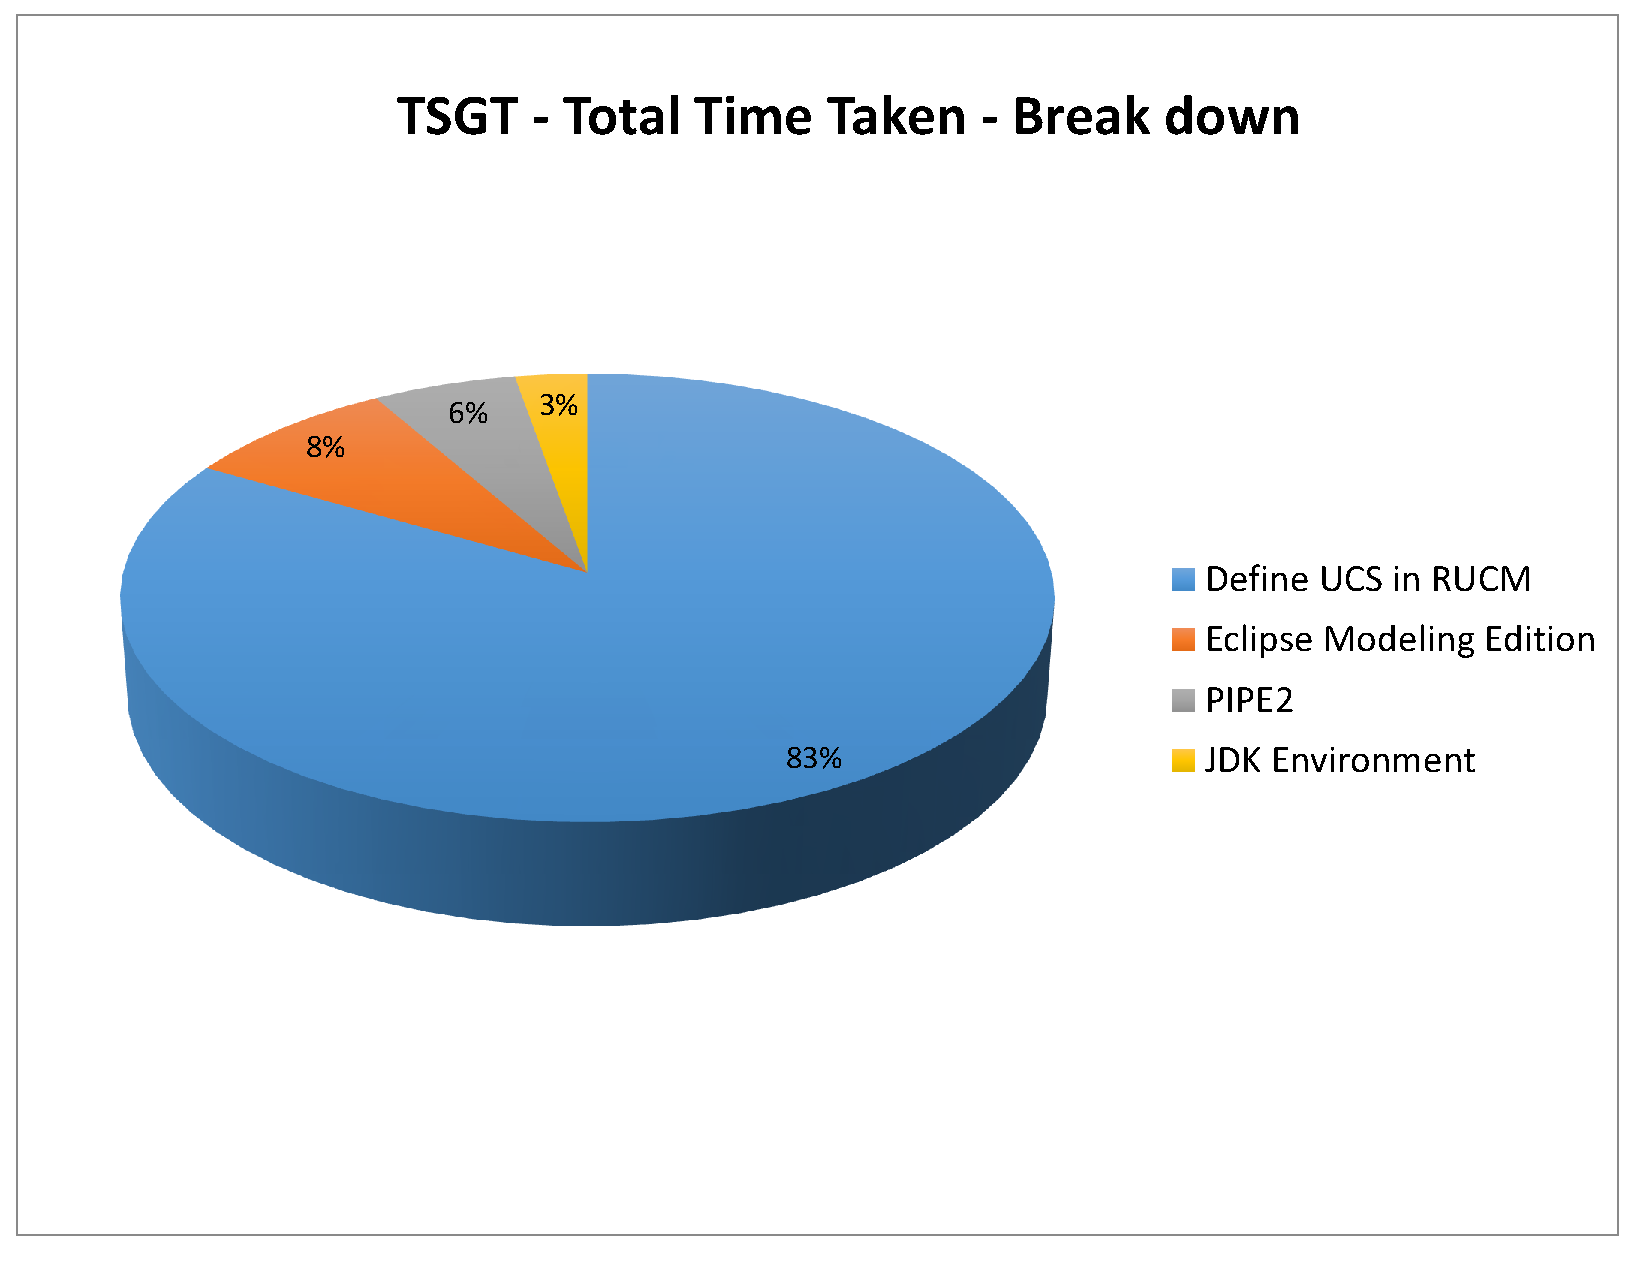
\includegraphics[scale=0.45]{content/images/Chapter6/figure4.pdf}
\caption{Breakdown of the time taken between different activities}
\label{fig:chap6fig4}
\end{figure}


The total time taken for test case generation in our tool is inclusive of the time taken to specify the \glspl{ucs} in \gls{rucm} template and to present them as input to our tool. This solely depends on the expertise of the user in \gls{rucm} template and also the experience in our tool. The time taken for test script generation after the input section is negligible. Figure \ref{fig:chap6fig4} shows how the total time taken for test script generation from each use case is split between different blocks in our tool. From the chart, it is obvious that the \gls{ucs} to \gls{rucm} template utilizes most of the time taken.


\begin{figure}[htb!]
\centering
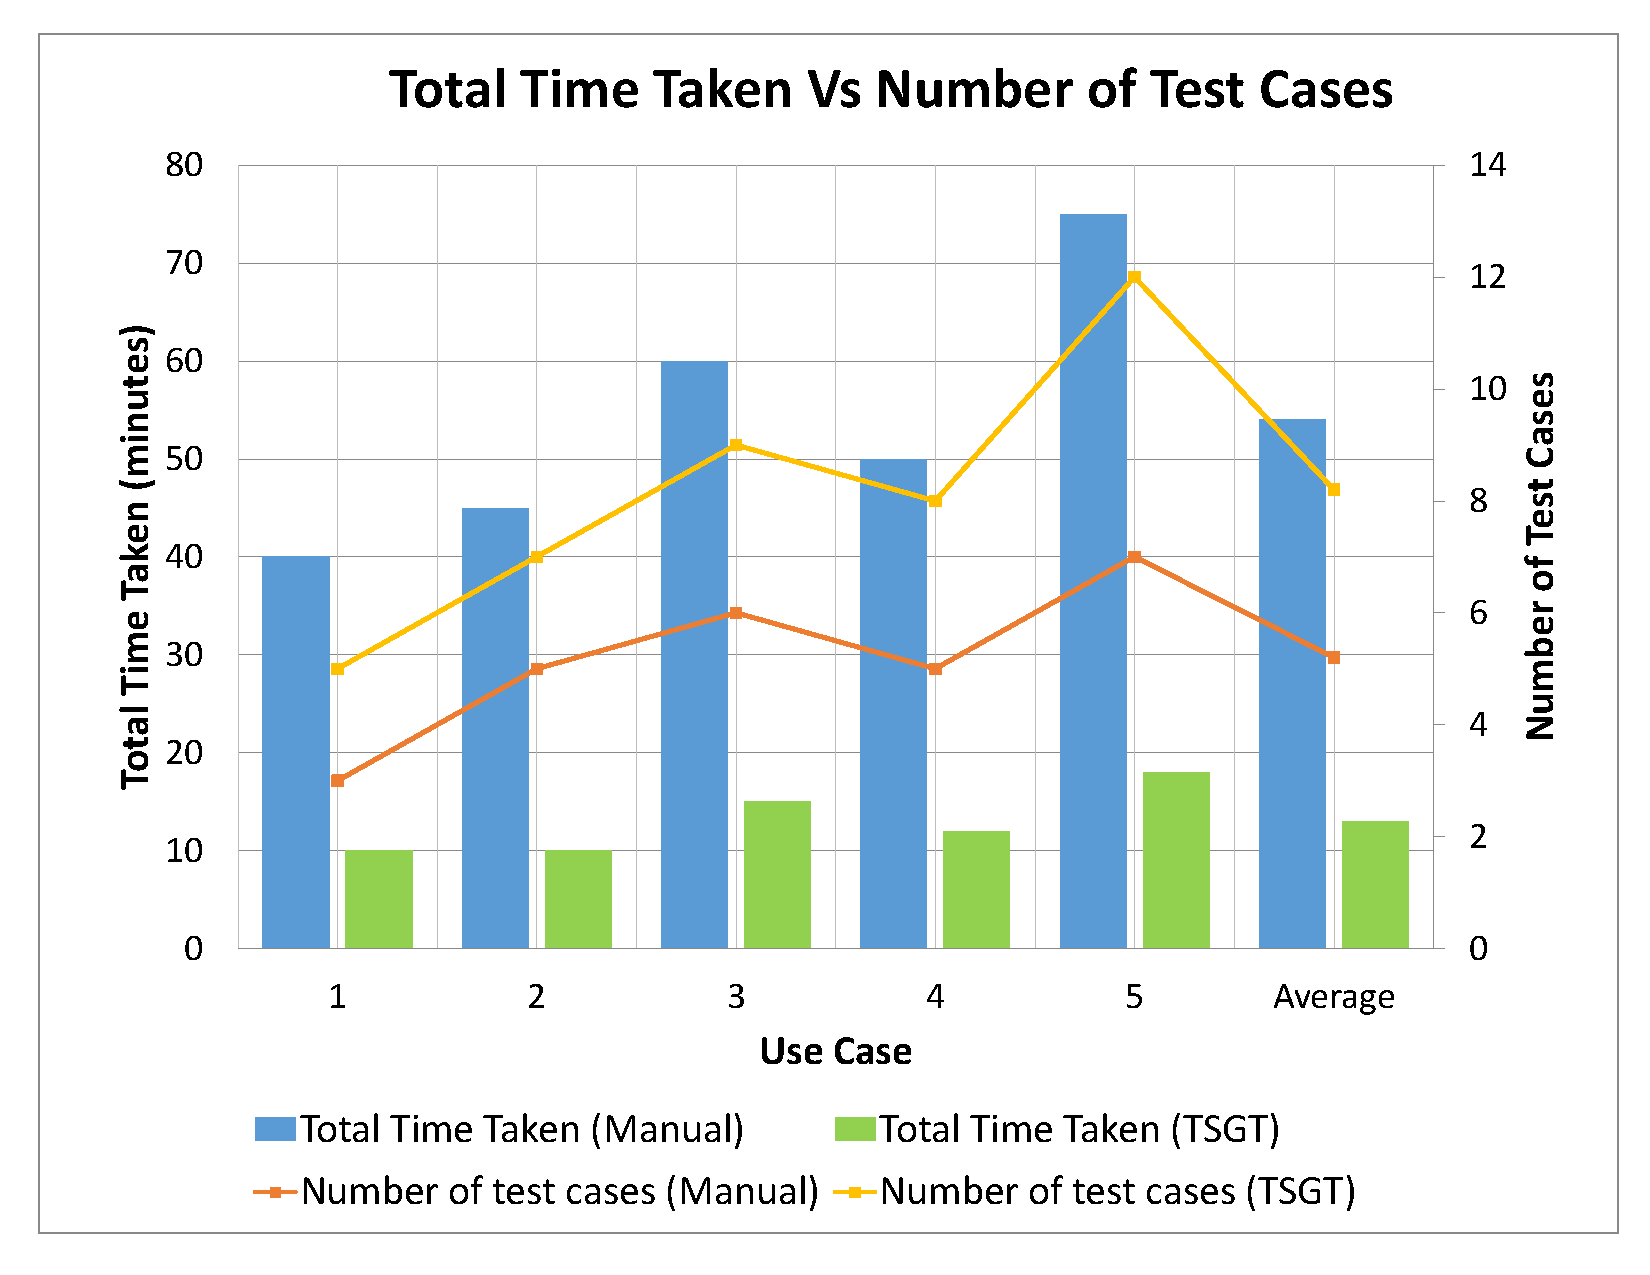
\includegraphics[scale=0.45]{content/images/Chapter6/figure5.pdf}
\caption{Relation between number of test cases and total time taken}
\label{fig:chap6fig5}
\end{figure}

The advantage of our tool is that the time taken to specify complex \glspl{ucs} does not add much to the total time taken, but produces more number of test cases. This scenario can be explained with the help of a graph as shown in Figure \ref{fig:chap6fig5}. By comparing Use Case 3 and Use Case 5, there is not much difference in the time required to specify the \glspl{ucs} but there is a drastic increase in the number of test cases that are generated thereby reducing the effort required to generate them. In the manual method, it can also be seen that more complex the use cases become, lesser the number of test cases identified. The average effort required to generate a test case will improve drastically when more number of complex use cases are evaluated.

\subsection{Summary}
This section summarizes the trends observed in the evaluation results and our tool characteristics. Evaluation criteria considering time and coverability have been compared between \gls{tsgt} and manual methods. The evaluation shows that \gls{tsgt} requires 85\% less effort than the manual method and it also provides 100\% coverability. 

Our tool has also been compared with other similar approaches in the research field and has been found to be good. Also, the limitations of our tool in reducing the effort required for each test case has been discussed and ways to improve them are suggested. From all the above discussions, it can be concluded that the automatic test case generation using \gls{tsgt} is definitely better than manual test case generation and other existing approaches. 